% --------------------------------------------
% Definição do tipo do documento e suas
% características.
% --------------------------------------------
\documentclass[
    12pt,                   % Tamanho da fonte.
    a4paper,                % Tipo de papel.
    sumario=tradicional,    % Tipo de sumário.
    brazil,                 % Linguagem principal do documento.
    oneside                 % Imprimir documento em um lado da folha.
]{abntex2}                  % Estilo do documento.

% --------------------------------------------
% Importação de configurações pessoais.
% --------------------------------------------
\usepackage{setup/packages}


%! Author = gabriel
%! Date = 5/17/21

% --------------------------------------------
% Insira o nome do(s) autor(es).
% Caso seja mais de um, insira \and entre os
% nomes de cada um.
% --------------------------------------------
\author{Gabriel Medeiros Lopes Carneiro}

% --------------------------------------------
% Insira o nome da universidade.
% --------------------------------------------
\university{Universidade Federal de Santa Catarina}

% --------------------------------------------
% Insira o nome do centro de ensino.
% --------------------------------------------
\educationcenter{Centro Tecnológico}

% --------------------------------------------
% Insira o nome do departamento de ensino.
% --------------------------------------------
\department{Departamento de Informática e Estatística}

% --------------------------------------------
% Insira o nome do curso ao qual pertence.
% --------------------------------------------
\course{Ciências da Computação}

% --------------------------------------------
% Afiliação do autor.
% -------------------------------------------- 
\affil{\printuniversity \\
        \printeducationcenter \\
        \printdepartment \\
        \printcourse}

%! Author = gabriel
%! Date = 5/17/21

% --------------------------------------------
% Insira o título do trabalho.
% --------------------------------------------
\title{Título}
% --------------------------------------------
% Caso o trablalho tenha subtítulo, descomente
% a linha abaixo.
% OBS.: NÃO APAGAR ":~" irá desconfigurar o arquivo.
% --------------------------------------------
\subtitle{:~Subtítulo (se houver)}

% --------------------------------------------
% Insira o tipo de trabalho do documento.
% --------------------------------------------
\worktype{Tipo do trabalho}

% --------------------------------------------
% Insira o local de apresentação do documento.
% --------------------------------------------
\local{Florianópolis, SC}

% --------------------------------------------
% Define a data do documento. Por padrão mostra
% apenas o ano, caso queira a data completa,
% substitua por \today.
% --------------------------------------------
\date{\the\year}

% --------------------------------------------
% Caso o trabalho possua um orientador,
% comente a linha abaixo.
% --------------------------------------------
\orientador[Professor:]{Nome completo do professor}

% --------------------------------------------
% Caso o documento possua um orientador,
% descomente a linha abaixo.
% --------------------------------------------
%\orientador{Nome completo do orientador}

% --------------------------------------------
% Caso o documento possua um coorientador,
% descomente a linha abaixo.
% --------------------------------------------
%\coorientador{Nome completo do coorientador}

% --------------------------------------------
% Substituir '[mestre/doutor] em título obtido'
% pelo grau adequado.
% --------------------------------------------
%\formation{mestre/doutor em título obtido}

% --------------------------------------------
% Substituir nome do curso pelo nome do curso.
% --------------------------------------------
%\program{Programa de Pós-Graduação em nome do curso}

% --------------------------------------------
% Caso precise do preâmbulo do documento,
% descomente as linhas abaixo. Ele deve conter,
% o tipo do documento, o objetivo, o nome da
% instituição e a área de concentração.
% --------------------------------------------
%\preambulo{
%    \printworktype~ submetida ao
%    \printprogram~ da \printuniversity~
%    para a obtenção do título de \printformation.
%}

% --------------------------------------------
% Definição de cores de hyperlinks
% e formatações do pdf.
% --------------------------------------------
\hypersetup{
    colorlinks=true,
    linkcolor=black,
    filecolor=magenta,
    urlcolor=blue,
    citecolor=black,
    pdfauthor=\theauthor,
    pdftitle=\thetitle,
    bookmarksopen=true,
}

% --------------------------------------------
% Início do documento.
% --------------------------------------------
% Aqui devem ser inseridas todas informações.
% --------------------------------------------
\begin{document}
    % --------------------------------------------
    % Inserção dos elementos pré-textuais.
    % --------------------------------------------
    % Capa, folha de rosto, ficha catalográfica,
    % errata, folha de aprovação, dedicatória,
    % agradecimentos, epígrafe, resumos,
    % lista de ilustrações, lista de tabelas,
    % lista de abreviaturas e siglas,
    % lista de símbolos e sumário.
    % --------------------------------------------
    %! Author = gabriel
%! Date = 5/17/21

% Logo da UFSC
%\begin{figure}
%    
\includegraphics[scale=0.2]{logo-ufsc}
%    \centering
%    \label{fig:logo-ufsc}
%\end{figure}

% Geração de Título

% --------------------------------------------
% Para usar título padrão latex, descomente
% a linha abaixo.
% --------------------------------------------
%\maketitle

% TODO: melhorar capa


% --------------------------------------------
% Geração da capa.
% --------------------------------------------
\printcoverufsc
%\printcover

% --------------------------------------------
% Geração da folha de rosto.
% --------------------------------------------
\printtitlepage

% --------------------------------------------
% Resumo do documento de acordo com padrões
% Latex. Caso queira de acordo com a ABNT,
% comente as linhas abaixo.
% --------------------------------------------
%\begin{abstract}
%    Write here.
%\end{abstract}

% --------------------------------------------
% Comentar linhas abaixo para não ter um
% resumo de acordo com a ABNT.
% --------------------------------------------
\begin{resumo}
    A bolsa de iniciação científica teve como foco de estudo computação quântica.
    Durante o período, duas linguagens de programação quântica foram estudadas, sendo elas Qiskit e Ket.
    Além disso, os principais algoritmos quânticos foram vistos, como, por exemplo, o algoritmo de busca de Grover, a estimativa de fase, busca de ordem, entre outros.
    Com os conhecimentos adquiridos também foi possível participar de um projeto de extensão relacionado a um simulador quântico.
\end{resumo}
\newpage

% --------------------------------------------
% Caso seja necessário um resumo em inglês,
% descomentar linhas abaixo.
% --------------------------------------------
%\begin{resumo}[Abstract]
%    Escreva o resumo em inglês aqui.
%\end{resumo}
%\newpage

% --------------------------------------------
% Lista de Figuras.
% --------------------------------------------
\listoffigures*
\newpage

% --------------------------------------------
% Lista de Tabelas.
% --------------------------------------------
%\listoftables*
%\newpage

% --------------------------------------------
% Geração do Sumário.
% --------------------------------------------
\tableofcontents*

    % --------------------------------------------
    % Inserção dos elementos textuais.
    % --------------------------------------------
    % Aqui devem ser inseridos todos os capítulos
    % e/ou seções do trabalho.
    % --------------------------------------------
    \chapter{Introdução}\label{ch:introducao}
    % --------------------------------------------
% Aqui você deve organizar as seções.
% --------------------------------------------
\chapter{Introdução}\label{ch:introducao}

\section{Motivação}\label{sec:Motivacao}
% --------------------------------------------
% Aqui você deve escrever o texto.
% --------------------------------------------
Escreva aqui.

\section{Justificativas}\label{sec:Justificativas}
% --------------------------------------------
% Aqui você deve escrever o texto.
% --------------------------------------------
Escreva aqui.\cite{einstein}

\section{Objetivos}\label{sec:Objetivos}
% --------------------------------------------
% Aqui você deve organizar as subsubseções.
% --------------------------------------------
\subsection{Objetivo Geral}\label{subsec:objetivo-geral}
% --------------------------------------------
% Aqui você deve escrever o texto.
% --------------------------------------------
Escreva aqui.

\subsection{Objetivos Específicos}\label{subsec:objetivos-especificos}
% --------------------------------------------
% Aqui você deve escrever o texto.
% --------------------------------------------


    % --------------------------------------------
    % Definição do estilo da bibliografia.
    % Deve estar comentado para padrão ABNT.
    % --------------------------------------------
    %\bibliographystyle{unsrt}

    % --------------------------------------------
    % Definição do arquivo da bibliografia.
    % --------------------------------------------
    \bibliography{aftertext/references}

    % --------------------------------------------
    % Inserção dos elementos pós-textuais.
    % --------------------------------------------
    % Glossário, apêndices, anexos e índice.
    % --------------------------------------------
    % --------------------------------------------
% Organização dos elementos pós-textuais.
% --------------------------------------------
\postextual

\anexos
\chapter{Certificado “Consciência da ciência ou sociedade sem ciência?”}\label{ch:certificado-consciencia-da-ciencia-ou-sociedade-sem-ciencia}

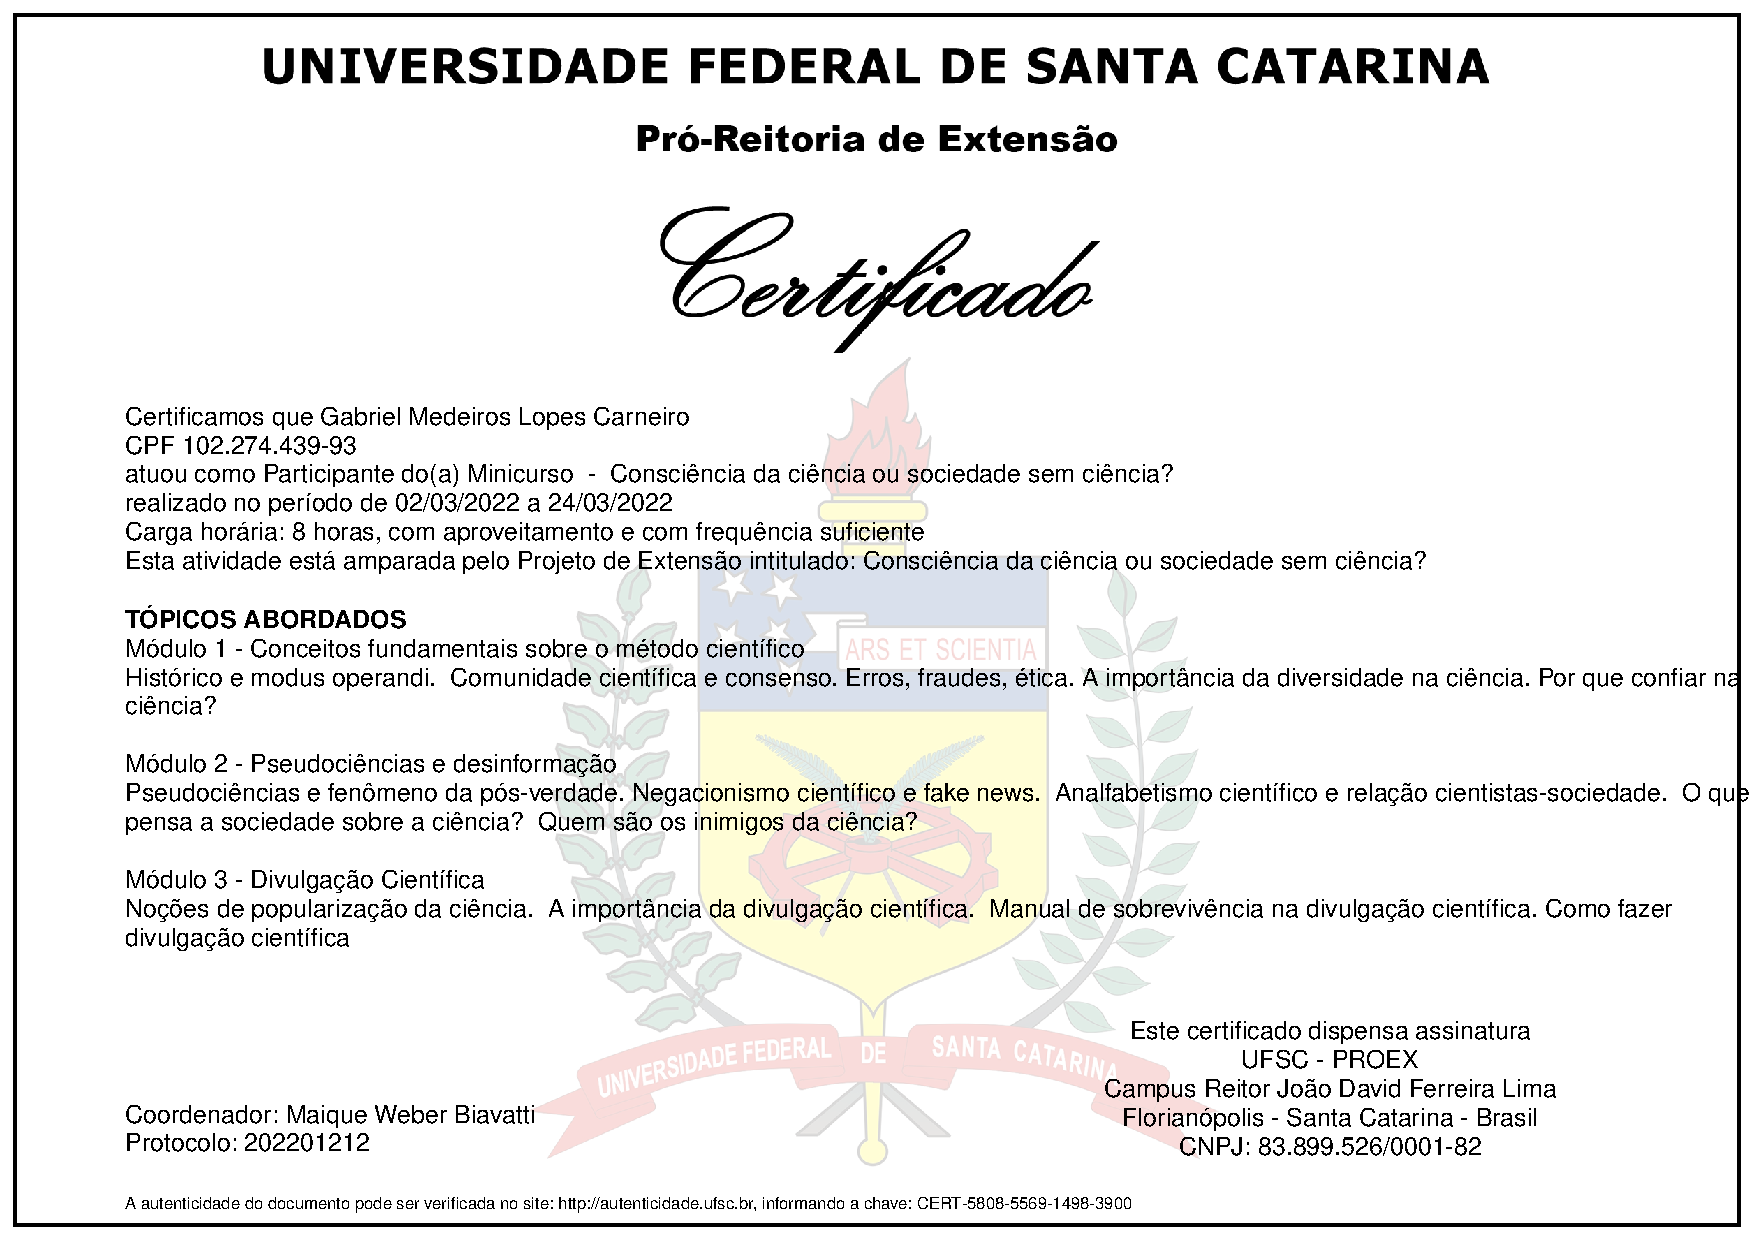
\includepdf{aftertext/minicurso-consciencia-ciencia}


\end{document}
% --------------------------------------------
% Final do documento. Não adicionar nada após.
% --------------------------------------------